\documentclass[border=8pt]{standalone}
\usepackage{amsmath,amssymb,bm}
\usepackage{xcolor}
\usepackage{tikz}
% --- one accent per nonet; every other tone is derived from it ---
\definecolor{P}{HTML}{49B7B1}
\definecolor{ink}{HTML}{1B1B2F}
\colorlet{band}{P!7!white}
\colorlet{lcol}{P!18!white}
\colorlet{rule}{P!45!white}
\colorlet{Pd}{P!80!white}
\begin{document}
\large
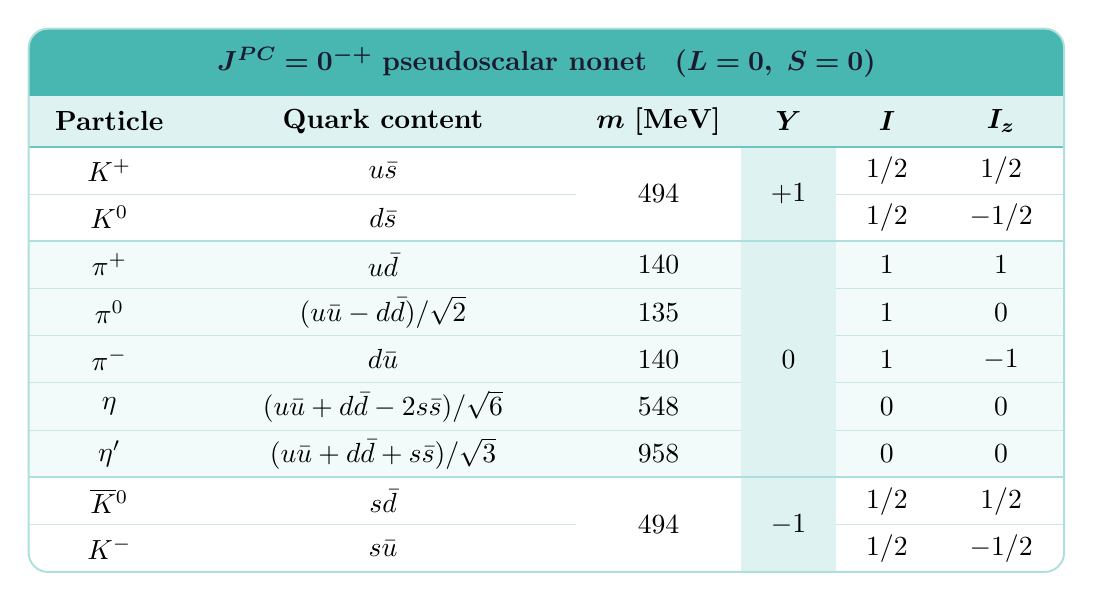
\begin{tikzpicture}
  \begin{scope}
    \clip[rounded corners=7pt] (0,0) rectangle (13.150,-6.900);
    \fill[P] (0,0) rectangle (13.150,-0.850);
    \fill[lcol] (0,-0.850) rectangle (13.150,-1.500);
    \fill[band] (0,-2.700) rectangle (13.150,-5.700);
    \fill[lcol] (9.050,-1.500) rectangle (10.250,-6.900);
  \end{scope}
  \draw[rule!70,line width=.35pt] (0.000,-2.100) -- (6.950,-2.100) (10.250,-2.100) -- (13.150,-2.100);
  \draw[rule,line width=.7pt] (0,-2.700) -- (13.150,-2.700);
  \draw[rule!70,line width=.35pt] (0.000,-3.300) -- (9.050,-3.300) (10.250,-3.300) -- (13.150,-3.300);
  \draw[rule!70,line width=.35pt] (0.000,-3.900) -- (9.050,-3.900) (10.250,-3.900) -- (13.150,-3.900);
  \draw[rule!70,line width=.35pt] (0.000,-4.500) -- (9.050,-4.500) (10.250,-4.500) -- (13.150,-4.500);
  \draw[rule!70,line width=.35pt] (0.000,-5.100) -- (9.050,-5.100) (10.250,-5.100) -- (13.150,-5.100);
  \draw[rule,line width=.7pt] (0,-5.700) -- (13.150,-5.700);
  \draw[rule!70,line width=.35pt] (0.000,-6.300) -- (6.950,-6.300) (10.250,-6.300) -- (13.150,-6.300);
  \draw[Pd,line width=.7pt] (0,-1.500) -- (13.150,-1.500);
  \draw[rule,line width=.7pt,rounded corners=7pt] (0,0) rectangle (13.150,-6.900);
  \node[text=ink,align=center] at (6.575,-0.425) {$\bm{J^{PC}=0^{-+}}\ \textbf{pseudoscalar nonet}\quad \bm{(L=0,\ S=0)}$};
  \node at (1.025,-1.175) {\textbf{Particle}};
  \node at (4.500,-1.175) {\textbf{Quark content}};
  \node at (8.000,-1.175) {$\bm{m}$ \textbf{[MeV]}};
  \node at (9.650,-1.175) {$\bm{Y}$};
  \node at (10.900,-1.175) {$\bm{I}$};
  \node at (12.350,-1.175) {$\bm{I_z}$};
  \node at (9.650,-2.100) {$+1$};
  \node at (9.650,-4.200) {$0$};
  \node at (9.650,-6.300) {$-1$};
  \node at (1.025,-1.800) {$K^+$};
  \node at (4.500,-1.800) {$u\bar s$};
  \node at (10.900,-1.800) {$1/2$};
  \node at (12.350,-1.800) {$1/2$};
  \node at (1.025,-2.400) {$K^0$};
  \node at (4.500,-2.400) {$d\bar s$};
  \node at (10.900,-2.400) {$1/2$};
  \node at (12.350,-2.400) {$-1/2$};
  \node at (1.025,-3.000) {$\pi^+$};
  \node at (4.500,-3.000) {$u\bar d$};
  \node at (10.900,-3.000) {$1$};
  \node at (12.350,-3.000) {$1$};
  \node at (1.025,-3.600) {$\pi^0$};
  \node at (4.500,-3.600) {$(u\bar u-d\bar d)/\sqrt2$};
  \node at (10.900,-3.600) {$1$};
  \node at (12.350,-3.600) {$0$};
  \node at (1.025,-4.200) {$\pi^-$};
  \node at (4.500,-4.200) {$d\bar u$};
  \node at (10.900,-4.200) {$1$};
  \node at (12.350,-4.200) {$-1$};
  \node at (1.025,-4.800) {$\eta$};
  \node at (4.500,-4.800) {$(u\bar u+d\bar d-2s\bar s)/\sqrt6$};
  \node at (10.900,-4.800) {$0$};
  \node at (12.350,-4.800) {$0$};
  \node at (1.025,-5.400) {$\eta'$};
  \node at (4.500,-5.400) {$(u\bar u+d\bar d+s\bar s)/\sqrt3$};
  \node at (10.900,-5.400) {$0$};
  \node at (12.350,-5.400) {$0$};
  \node at (1.025,-6.000) {$\overline{K}{}^0$};
  \node at (4.500,-6.000) {$s\bar d$};
  \node at (10.900,-6.000) {$1/2$};
  \node at (12.350,-6.000) {$1/2$};
  \node at (1.025,-6.600) {$K^-$};
  \node at (4.500,-6.600) {$s\bar u$};
  \node at (10.900,-6.600) {$1/2$};
  \node at (12.350,-6.600) {$-1/2$};
  \node at (8.000,-2.100) {$494$};
  \node at (8.000,-3.000) {$140$};
  \node at (8.000,-3.600) {$135$};
  \node at (8.000,-4.200) {$140$};
  \node at (8.000,-4.800) {$548$};
  \node at (8.000,-5.400) {$958$};
  \node at (8.000,-6.300) {$494$};
\end{tikzpicture}
\end{document}
